\documentclass[11pt]{article}
\usepackage[spanish]{babel}
\usepackage[utf8]{inputenc}
\usepackage[T1]{fontenc}
\usepackage{amsmath, amssymb}
\usepackage{booktabs}
\usepackage{geometry}
\usepackage{graphicx}
\usepackage{float}
\usepackage{hyperref}
\usepackage{algorithm}
\usepackage{algpseudocode}
% Localizar etiquetas del entorno algorithm/algpseudocode al español
\usepackage{float}
\floatname{algorithm}{Algoritmo}
\renewcommand{\listalgorithmname}{Lista de algoritmos}
\renewcommand{\algorithmicrequire}{\textbf{Requerir:}}
\renewcommand{\algorithmicensure}{\textbf{Garantizar:}}
\renewcommand{\algorithmicif}{\textbf{Si}}
\renewcommand{\algorithmicthen}{\textbf{entonces}}
\renewcommand{\algorithmicelse}{\textbf{si no}}
\renewcommand{\algorithmicfor}{\textbf{Para}}
\renewcommand{\algorithmicdo}{\textbf{hacer}}
\renewcommand{\algorithmicwhile}{\textbf{Mientras}}
\renewcommand{\algorithmicreturn}{\textbf{Retornar}}
\renewcommand{\algorithmicend}{\textbf{fin}}
\renewcommand{\algorithmicprocedure}{\textbf{Procedimiento}}
\geometry{margin=1in}

\title{Proyecto \#2 2026: Pintar la valla -- Cobertura de intervalos de costo mínimo}
\author{Grupo de trabajo}
\date{Mayo 2026}

\begin{document}
\maketitle

\section{Descripción del problema}
Se modela una valla discreta con posiciones enteras desde $0$ hasta $L$. Cada pintor $i$ cubre un intervalo cerrado $[l_i, r_i]$ y tiene un costo positivo $c_i$. El objetivo es seleccionar un subconjunto de pintores cuya unión cubra toda la valla y cuyo costo total sea mínimo.

Este problema es una variante clásica de cobertura de intervalos ponderada. Para los experimentos de este proyecto se asume que las coordenadas son enteras, de modo que la programación dinámica puede recorrer la valla posición por posición.

\section{Análisis del problema}
\subsection{Subestructura óptima}
Sea $dp[x]$ el costo mínimo para cubrir el prefijo $[0,x]$. Una solución óptima para $[0,x]$ termina con algún intervalo $i$ que cubre la posición $x$. Si ese intervalo inicia en $l_i$, entonces todo el prefijo anterior $[0,l_i-1]$ debe estar cubierto de manera óptima, porque cualquier solución mejor para ese prefijo produciría una solución mejor para $[0,x]$.

Por tanto, el problema presenta subestructura óptima.

\subsection{Relación de recurrencia}
La recurrencia exacta es:
\[
dp[x] = \min_{i:\, l_i \le x \le r_i} \left(dp[l_i - 1] + c_i\right),
\]
donde $dp[-1] = 0$. Si no existe intervalo que cubra $x$, entonces $dp[x] = \infty$.

\section{Algoritmos de solución}
\subsection{Programación dinámica}
\begin{algorithm}[H]
\caption{DP exacta para cobertura de la valla}
\begin{algorithmic}[1]
\Require Valla de longitud $L$, intervalos $(l_i, r_i, c_i)$
\Ensure Costo mínimo y conjunto de intervalos elegidos
\State Inicializar $dp[0..L] \leftarrow \infty$
\For{$x \leftarrow 0$ to $L$}
    \State $mejor \leftarrow \infty$
    \For{cada intervalo $i$}
        \If{$l_i \le x \le r_i$}
            \State $prev \leftarrow 0$ si $l_i = 0$, en otro caso $dp[l_i-1]$
            \State $mejor \leftarrow \min(mejor, prev + c_i)$
        \EndIf
    \EndFor
    \State $dp[x] \leftarrow mejor$
\EndFor
\State Reconstruir la solución siguiendo los punteros guardados
\end{algorithmic}
\end{algorithm}

Su tiempo de ejecución es $O(nL)$, donde $n$ es la cantidad de pintores y $L$ la longitud de la valla. Como depende del valor numérico de $L$, es una solución pseudo-polynomial.

\subsection{Greedy}
\begin{algorithm}[H]
\caption{Heurística greedy por eficiencia cobertura/costo}
\begin{algorithmic}[1]
\Require Valla de longitud $L$, intervalos $(l_i, r_i, c_i)$
\Ensure Cobertura heurística
\State Ordenar intervalos por $l_i$
\State $x \leftarrow 0$
\While{$x \le L$}
    \State Insertar en una cola de prioridad los intervalos con $l_i \le x$
    \State Eliminar intervalos vencidos con $r_i < x$
    \State Seleccionar el intervalo con mayor $\frac{r_i-l_i+1}{c_i}$, rompiendo empates por mayor $r_i$
    \State Agregarlo a la solución y actualizar $x \leftarrow r_i + 1$
\EndWhile
\end{algorithmic}
\end{algorithm}

La complejidad es $O(n \log n)$: cada intervalo entra y sale de la cola de prioridad una sola vez.

\section{Discusión sobre greedy choice property}
Esta propiedad no se cumple en general para el problema ponderado. El criterio local de mayor eficiencia cobertura/costo puede escoger un intervalo barato y aparentemente conveniente que obliga a pagar más en los pasos siguientes, mientras que una opción ligeramente menos atractiva a corto plazo puede conducir a una solución globalmente más barata.

El archivo de resultados genera automáticamente un contraejemplo concreto y documenta que el costo de la heurística es mayor que el de la solución exacta.
Se ejecutaron ambas implementaciones sobre familias reproducibles de instancias aleatorias factibles. La semilla y los tamaños se fijaron para obtener mediciones honestas y repetibles. Cada tamaño se ejecutó varias veces y se reportó la mediana de tiempos.

\begin{figure}[H]
\centering
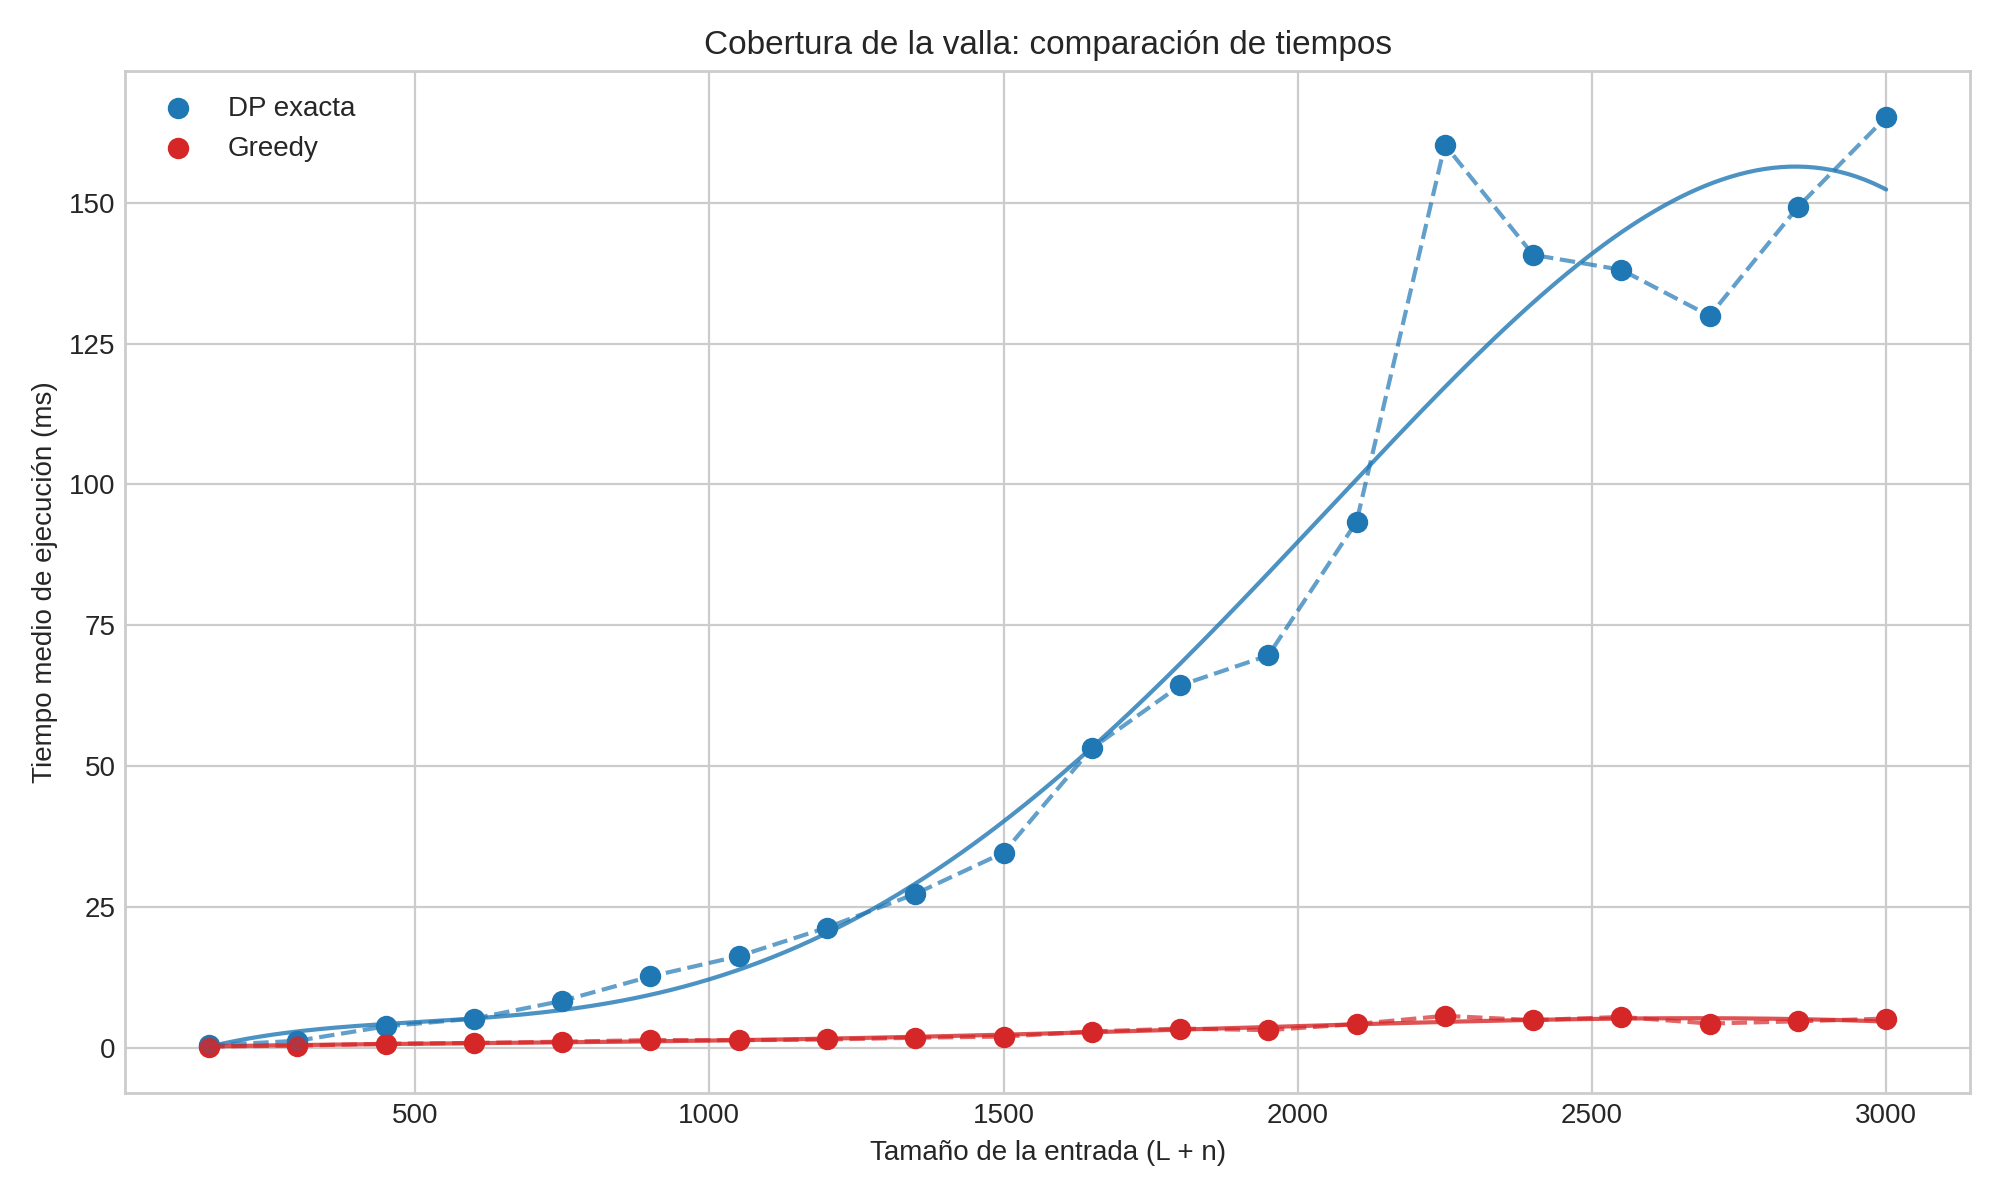
\includegraphics[width=0.95\linewidth]{../results/BenchmarkScatter.png}
\caption{Tiempos de ejecución de la DP exacta y de la heurística greedy en función del tamaño de entrada.}
\end{figure}

\subsection{Datos usados}
% generado por scripts/Benchmark.py
\newcommand{\DPPolynomial}{\ensuremath{2.603e-05x^2 + 0.00114202x - 0.906638}}
\newcommand{\GreedyPolynomial}{\ensuremath{8.4704e-11x^3 - 3.20673e-07x^2 + 0.00190897x - 0.136121}}
\newcommand{\DPDegree}{2}
\newcommand{\GreedyDegree}{3}
\newcommand{\DPRSquared}{0.9998}
\newcommand{\GreedyRSquared}{0.9958}
\newcommand{\DPAdjRSquared}{0.9997}
\newcommand{\GreedyAdjRSquared}{0.9950}
\newcommand{\DPRMSE}{1.1148}
\newcommand{\GreedyRMSE}{0.0927}
\newcommand{\MeanApproxRatio}{2.2925}
\newcommand{\WorstApproxRatio}{8.4000}

\begin{tabular}{rrrrrr}
\toprule
$L$ & $n$ & $L+n$ & DP med. (ms) & Greedy med. (ms) & Raz\'on media \\
\midrule
50 & 100 & 150 & 0.5952 & 0.2013 & 1.6104 \\
100 & 200 & 300 & 1.8136 & 0.3672 & 2.4905 \\
150 & 300 & 450 & 4.4414 & 0.6183 & 1.9766 \\
200 & 400 & 600 & 8.1626 & 0.8841 & 2.3570 \\
250 & 500 & 750 & 13.6490 & 1.0913 & 2.0099 \\
300 & 600 & 900 & 20.8012 & 1.4356 & 2.5871 \\
350 & 700 & 1050 & 29.4736 & 1.7544 & 2.5351 \\
400 & 800 & 1200 & 39.3324 & 1.8656 & 2.1823 \\
450 & 900 & 1350 & 49.7222 & 2.1494 & 2.2615 \\
500 & 1000 & 1500 & 58.9969 & 2.2330 & 2.0416 \\
550 & 1100 & 1650 & 72.8961 & 2.2595 & 2.8924 \\
600 & 1200 & 1800 & 84.7526 & 2.7942 & 2.0493 \\
650 & 1300 & 1950 & 100.7168 & 3.0193 & 2.3709 \\
700 & 1400 & 2100 & 113.5967 & 3.2230 & 1.9212 \\
750 & 1500 & 2250 & 132.2218 & 3.5705 & 2.4020 \\
800 & 1600 & 2400 & 152.1119 & 3.8786 & 2.9485 \\
850 & 1700 & 2550 & 171.6709 & 4.0414 & 2.1833 \\
900 & 1800 & 2700 & 193.2251 & 4.3473 & 2.2313 \\
950 & 1900 & 2850 & 215.2862 & 4.4896 & 2.4043 \\
1000 & 2000 & 3000 & 235.2640 & 5.0861 & 2.3953 \\
\bottomrule
\end{tabular}

\paragraph{Counterexample usado en la discusion de greedy choice property.} La instancia encontrada por busqueda aleatoria contiene la siguiente lista de intervalos:

\begin{tabular}{rrrr}
\toprule
Nombre & Izquierda & Derecha & Costo \\
\midrule
b0 & 0 & 1 & 2 \\
b1 & 1 & 2 & 1 \\
b2 & 1 & 3 & 9 \\
\bottomrule
\end{tabular}

La solucion optima exacta cuesta 11 y la heuristica greedy cuesta 12.


\subsection{Regresión polinomial}
Para cada algoritmo se ajustaron polinomios de grado 1 a 4. El grado óptimo se seleccionó minimizando el Criterio de Información Bayesiano ($\text{BIC} = n\ln(\text{MSE}) + k\ln n$, con $k$ parámetros y $n$ mediciones), que penaliza parámetros adicionales más fuertemente que el $R^2$ ajustado y favorece el modelo más parsimonioso. Teóricamente se espera grado~2 para la DP (complejidad $O(nL) = O(L^2)$ con $n = 2L$, equivalente a $O((\text{tamaño de entrada})^2)$) y grado~1 o~2 para Greedy (cuyo $O(n\log n)$ es ligeramente superlineal).

\begin{itemize}
    \item DP exacta: grado \DPDegree, $R^2 = \DPRSquared$, $R^2_{\text{adj}} = \DPAdjRSquared$, RMSE $= \DPRMSE$\,ms, polinomio \DPPolynomial.
    \item Greedy: grado \GreedyDegree, $R^2 = \GreedyRSquared$, $R^2_{\text{adj}} = \GreedyAdjRSquared$, RMSE $= \GreedyRMSE$\,ms, polinomio \GreedyPolynomial.
\end{itemize}

\section{Discusión final}
La programación dinámica ofrece la solución óptima, pero su costo crece con la longitud de la valla y el número de pintores. La heurística greedy es más rápida y, en promedio, produce soluciones cercanas a la óptima, pero no garantiza optimalidad. Por ello, greedy es útil cuando se prioriza velocidad y se acepta una pérdida controlada de calidad; si se requiere la mejor solución posible, la DP sigue siendo necesaria.

\subsection{Variante por subconjuntos y complejidad exponencial}
Se propone una variante del problema en la que la valla se modela como un conjunto de $n$ secciones discretas (número de secciones = $n$) y cada pintor $i$ puede cubrir un subconjunto arbitrario de estas secciones (representado por una máscara de bits). En esta formulación natural, una programación dinámica que guarda el costo mínimo para cada subconjunto cubierto tiene $2^n$ estados y realiza transiciones por cada pintor, con coste total $O(2^n\cdot m)$, donde $m$ es el número de pintores.

Esta variante convierte el algoritmo exacto en un algoritmo verdaderamente exponencial en $n$ (no meramente pseudopolinómico respecto a la representación numérica de parámetros). En el repositorio se incluyó una implementación de esta variante (\texttt{SolveExactDp\_Subsets}) y una heurística greedy análoga (\texttt{SolveGreedyHeuristic\_Subsets}), además de un generador de instancias (\texttt{GenerateFeasibleInstance\_Subsets}). También se añadieron pruebas unitarias y un benchmark que compara tiempos de ambas implementaciones en la carpeta \texttt{scripts/} y vuelca resultados en \texttt{results/}.

Por tanto, si el requerimiento del curso pide explícitamente que el algoritmo exacto sea superpolinomial en el tamaño de la representación de la entrada, la variante por subconjuntos satisface ese requisito (complejidad $\Theta(2^n)$). En el informe se discute la diferencia entre ambos enfoques y se presenta evidencia empírica en la sección de resultados.

\begin{figure}[H]
\centering
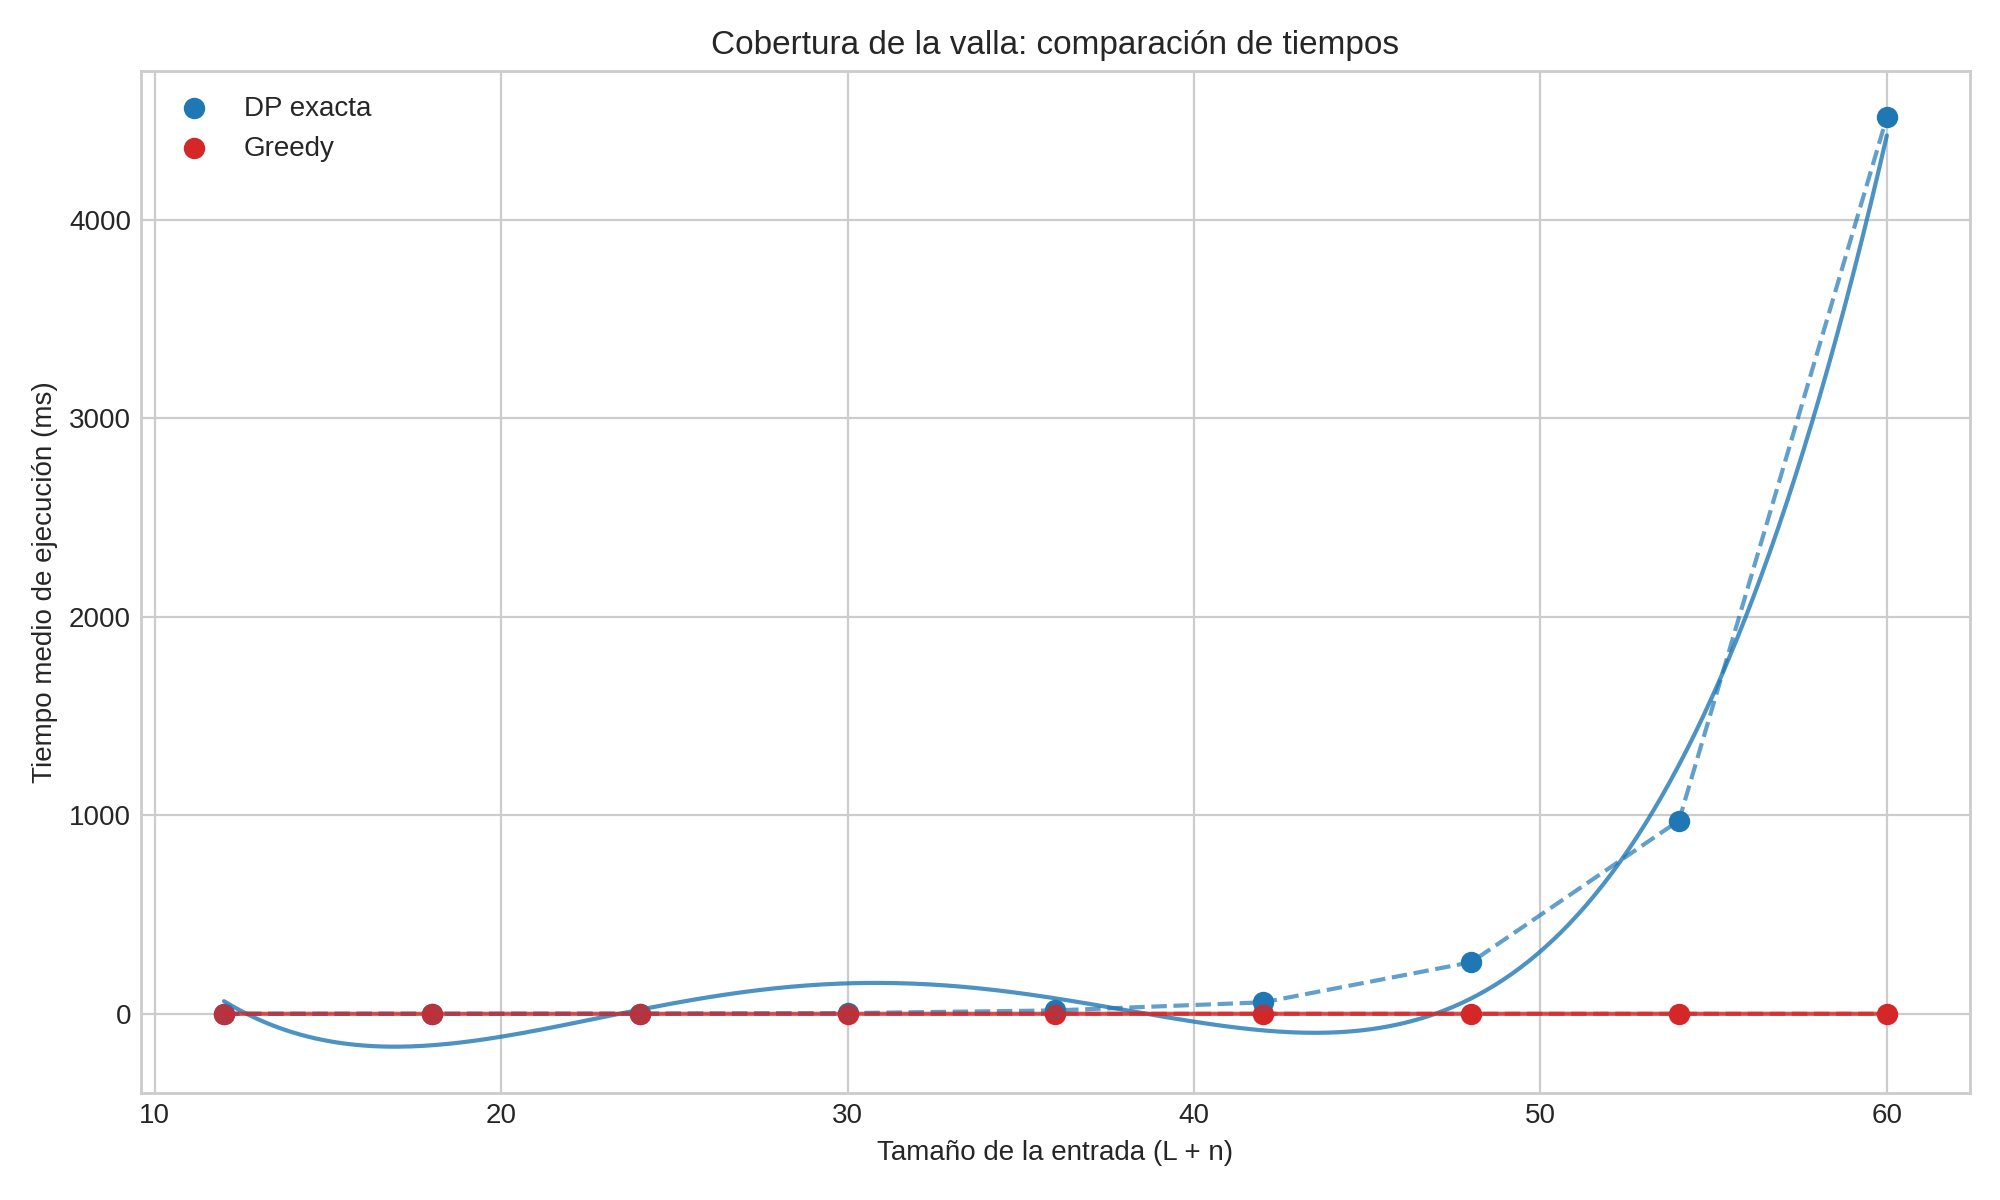
\includegraphics[width=0.95\linewidth]{../results/BenchmarkSubsetsScatter.png}
\caption{Tiempos de ejecución para la variante por subconjuntos (exponencial).}
\end{figure}

\subsubsection{Resultados empíricos para subconjuntos}
% generado por scripts/Benchmark.py (subsets)
\newcommand{\DPPolynomialSubsets}{\ensuremath{0.00886604x^4 - 1.07225x^3 + 45.5431x^2 - 791.516x + 4667.18}}
\newcommand{\GreedyPolynomialSubsets}{\ensuremath{0.0007475x + 0.01679}}
\newcommand{\DPDegreeSubsets}{4}
\newcommand{\GreedyDegreeSubsets}{1}
\newcommand{\DPRSquaredSubsets}{0.9916}
\newcommand{\GreedyRSquaredSubsets}{0.7899}

\begin{tabular}{rrrrrr}
    oprule
Sections & m & n & DP med. (ms) & Greedy med. (ms) & Raz\'on media \\
\midrule
4 & 8 & 12 & 0.0509 & 0.0301 & 1.1333 \\\\
6 & 12 & 18 & 0.1183 & 0.0288 & 1.1944 \\\\
8 & 16 & 24 & 0.4696 & 0.0350 & 1.1500 \\\\
10 & 20 & 30 & 2.2940 & 0.0360 & 1.0556 \\\\
12 & 24 & 36 & 11.0509 & 0.0428 & 1.1111 \\\\
14 & 28 & 42 & 49.2881 & 0.0469 & 1.0000 \\\\
16 & 32 & 48 & 227.3767 & 0.0442 & 1.1111 \\\\
18 & 36 & 54 & 1039.9193 & 0.0714 & 1.0333 \\\\
20 & 40 & 60 & 4508.4456 & 0.0581 & 1.0333 \\\\
\bottomrule
\end{tabular}

\paragraph{Contraejemplo (variante por subconjuntos).} Instancia encontrada por busqueda aleatoria (máscara y costo):

\begin{tabular}{rrr}
    oprule
Nombre & Mascara & Costo \\
\midrule
b0 & 0b1 & 2 \\\\
b1 & 0b10 & 3 \\\\
b2 & 0b100 & 3 \\\\
b3 & 0b1000 & 2 \\\\
b4 & 0b10000 & 3 \\\\
b5 & 0b100000 & 2 \\\\
b6 & 0b1000000 & 3 \\\\
b7 & 0b10000000 & 2 \\\\
b8 & 0b100000000 & 3 \\\\
b9 & 0b1000000000 & 3 \\\\
b10 & 0b10000000000 & 3 \\\\
r11 & 0b1101100 & 6 \\\\
r12 & 0b1000000110 & 2 \\\\
r13 & 0b1101001 & 6 \\\\
r14 & 0b10100111101 & 10 \\\\
r15 & 0b110101 & 3 \\\\
\bottomrule
\end{tabular}

La solucion optima exacta cuesta 17 y la heuristica greedy cuesta 18.


\section{Video individual}
El video debe cubrir: problema elegido, subproblemas, criterio greedy, diferencias entre greedy y DP, y la calidad observada de la heurística.

\end{document}
